\documentclass[tikz]{standalone}
\usepackage{amsmath,amssymb}
\usetikzlibrary{patterns}


\newcommand{\V}[1]{\vec{\mathbf{#1}}}
\tikzset{wristwatchnode/.style={scale=0.7}}
\tikzset{myaxis/.style={->}}
\tikzset{myvec/.style={very thick,->,shorten >=.5mm}}
\tikzset{mynode/.style={scale=0.7}}

\begin{document}
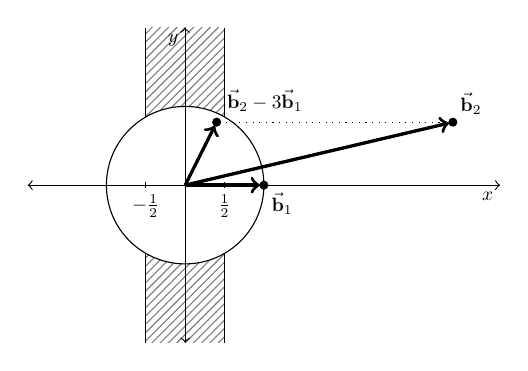
\begin{tikzpicture}
	\clip (-2,-2) rectangle (4,2);

	\fill[pattern color=black!50,pattern=north east lines] (.5,-2) -- (.5,2) -- (-.5,2) -- (-.5,-2);
	\draw (.5,-2) -- (.5,2) (-.5,-2) -- (-.5,2);
	\draw[fill=white] (0,0) circle (1cm);

	\draw[myaxis] (0,0) -- (-2,0);
	\draw[myaxis] (0,0) -- (0,-2);
	\draw[myaxis] (0,0) -- (4,0) node[mynode,below left] {\(x\)};
	\draw[myaxis] (0,0) -- (0,2) node[mynode,below left] {\(y\)}; % axis lines

	% \draw[gray,dashed,-] (-2,0) -- (2,0) (0,-2) -- (0,2); % axis lines

	\draw[fill=black] (1,0) circle (.5mm) (.4,.8) circle (.5mm) (3.4,.8) circle (.5mm);

	\draw[dotted] (3.4,.8) -- (.4,.8);

	\draw[myvec] (0,0) -- (1,0) node[wristwatchnode,below right] {$\V b_1$};
	\draw[myvec] (0,0) -- (.4,.8) node[wristwatchnode,above right=.5mm] {$\V b_2 - 3 \V b_1$};
	\draw[myvec] (0,0) -- (3.4,.8) node[wristwatchnode,above right] {$\V b_2$};

	\draw (-.5,-.04) -- (-.5,.04) node[wristwatchnode,below=0.1cm] {$-\frac12$};
	\draw (.5,-.04) -- (.5,.04) node[wristwatchnode,below=0.1cm] {$\frac12$};
\end{tikzpicture}
\end{document}
